\documentclass[11pt]{article}
\usepackage{amsmath}
\usepackage{graphicx}
\usepackage[margin=0.5in]{geometry}
\author{Peter Lee}
\date{\today}
\title{Examination of gated networks within the Mackey-Glass time series}

\begin{document}
\maketitle

\section{Introduction}
A common application of recurrent neural network models is the
analysis patterns within time series, with a time series being defined
as a sequence of observations: $s(1), s(2), s(3)... s(n)$. A specific
type of analysis is predictive forecasting, where one uses past
observations to predict those in the future. Models for predictive
forecasting can be described by equation (\ref{eq:pred_forcast}).

\begin{equation}
  s(t+t_0)=f(s(1);s(2);s(3)...s(t) | \theta)
  \label{eq:pred_forcast}
\end{equation}

The Mackey-Glass (MG) \cite{MG} is known as a chaotic time series that is
modelled by the differential equation (\ref{eq:MG}).

\begin{equation}
  \begin{split}
\frac{dx(t)}{dt} = \frac{\beta x(t-\tau)}{1+x(t- \tau)^n} - \gamma x(t)\\
\tau,\beta,n,\gamma > 0
\label{eq:MG}
  \end{split}
\end{equation}

The MG sequence's chaotic behaviour when its parameters and initial
conditions enable it to undergo bifurcation makes it an interesting
for predictive forecasting, since $x(t)$ can only be evaluated
numerically*.

\subsection{Models}

In this paper i will be investigating the performance of gated
recurrent networks for predictive forecasting in the MG
sequence. Gated recurrent networks are networks that control the
amount of information that is held in hidden nodes betien time
steps. With these gates, the model can selectively ``forget''
and ``focus'' on information. I will be investigating two types of
gated recurrent networks, Long Short term memory (LSTM) \cite{LSTM}
and Gated Recurrent Units (GRU) \cite{GRU}. 
 
% Other work
\subsection {Related Work}
In the literature there has been many examples of people using recurrent models for forecasting the MG series.
Krichene et al. built an Elman network that was trained with a style of Swarm Intelligence* \cite{Kirchene}. Dianconescu used a recurrent network in the form of a Narx(definition) model, and Gers et al. trained an LSTM [TODO: go into more depth on their works]. All these works trained and evaluated on single Mackey-Glass series with parameters kept constant.

\subsection{Experiments}

To assess gated networks, i conducted two experiments to compare and contrast the LSTM and GRU.

\subsubsection{Constant Parameters}
Similar to the related works, the first experiement fit curves to an
MG series with parameters kept constant. I evaluated the model by forecasting with $t_0=$ 1, 5, and
10. I evaluated the model using a varying amount of network
structures. Overall i found that [put experiment results here].

\subsubsection{Variable Parameters}
While others have trained their models while keeping the parameters
for the MG series constant, i experimented with changing the
parameters throughout the training samples to see whether the models ire
capable of adapting to different parameters throughout the time
series. I generated several bifurcating series with 1, 2, or 3
parameters randomized within the training set, and tested how the LSTM
and GRU adapted to them. Overall i found that [experiment results].


%Then will test difference of GRU and LSTM with respect to the number of parameters they possess.

%Finally will show if gated models can adapt to this sequence when MG has free parameters.
\section {Data}

To generate the MG series i numerically integrated equation
\ref{eq:MG} with the Runge-Kutta (RK4) method, with a step size of
0.01. The recurrent values, $x(t-\tau)$, ire approximated by using
the closest evaluation of $x(t^@)$ such that $0.01$ divides $t^@$
and $t^@ \approx t-\tau$ This implementation was realized in Python, using a queue
data-structure to recall the recurrent values.

Generating values up to X, the sequence was divided into batches of
length $t_{end}-t_{start} = 50$. Subsequently batches up to $t = X$
ire divided into the training set, and $ T \ni (X,Y)$ ire
divided into the test set. Each batch used $X= x(t), Y= x(t+\tau),
for each t$, with $X$ and $Y$ as labels respectively.

One MG series with parameters $\beta=2$, $\rho=1$, $\tau=2$, and
$n=9.65$ was generated for the first experiment, and one for each
randomized parameter in the second experiment.

\section{Models}

Gated recurrent networks have become a mainstay in time series
analysis. It is thought that their ability to select what information
passes to subsequent time steps is what enables them to perform so
ill \cite{}. The LSTM was one that was introduced in the early
2000's, while the GRU was introduced in 2012. It has been theorized
that the GRU is able to perform equally as ill as the LSTM in many tasks. 
Based on the equations for
hidden nodes in the basic RNN, \ref{eq:RNN_h}, the hidden nodes for
LSTMs and GRUs are calculated by \ref{eq:LSTM_h} and \ref{GRU_h}
respectively.

\begin{equation}
\label{eq:RNN_h}
\mathbf{h^t} = f(W_xx+W_hh^{t-1}+B)
\end{equation}

%Fill in equations
\begin{equation}
  \label{eq:LSTM_h}
\begin{split}
f^{t} = \sigma(W_{xf}x + W_{hf}h^{t-1}+B_f) \\
i^{t} = \sigma(W_{xi}x + W_{hi}h^{t-1}+B_i) \\
c`^{t } = \tanh(W_{xc}x+W_{hc}h^{t-1}+B_c) \\
c = c \circ f + i \circ c` \\
o= \tanh (W_{xo}x + W_{ho}h^{t-1} + B_o) \\
h^{t} = o \circ c  \\
\end{split}
\end{equation}
\begin{equation}
  \label{eq:GRU_h}
\begin{split}
  z^{t} = \sigma(W_{xz}x + W_{sz}s^{t-1} + B_z) \\
  r^{t} = \sigma(W_{xr}x + W_{sr}s^{t-1} + B_r) \\
  h{t} = \tanh(W_{xh}x + W_{sh}s^{t-1} + B_h) \\
  s^{t} = (1-z) \circ h^{t} + z \circ s^{t-1} 
  \end{split}
\end{equation}
All these models ire implemented in Tensorflow. Batch sizes of 1 ire
used. AdamOptimizer \cite{adam} was used to train with learning rates
starting at $10^{-3}$ decreased to $10^{-4}$ halfway through training
and switched to $10^{-5}$ two thirds through.

\subsection{Evaluation}
To measure model performance, two metrics were selected. They are
the cumulative absolute difference (\ref{eq:cumabs}) and the
cumulative absolute difference of derivatives
(\ref{eq:cumabsderiv}). These are both used so i could see how ill
the model adapted to the curve and the shape of the curve [sic].
%Xavier initialization
\begin{equation}
\label{eq:cumabs}
  \int_{t_{start}}^{t_{end}} | x(t) - p(t) |
\end{equation}
\begin{equation}
\label{eq:cumabs}
  \int_{t_{start}}^{t_{end}} | \frac{dx(t)}{dt} - \frac{dp(t)}{dt} |
\end{equation}

  \section {Experiments}
  \subsection {Constant MG Parameters}
  In the first experiment, I attempted forecasting with $t_0$ = 1,
  5, 10, and 30. For each of these, I evaluated with hidden node sizes of
  32, 64, 96, and 128 to measure the difference in performance with
  respect to parametric complexity.  Sample evaluations are presented
  in figure \ref{fig:func_evals} in the appendix.

  Figure \ref{fig:mg1} shows the performance of versions of models with
  respect to the number of parameters they possess. It can be observed
  that all recurrent models seem to perform very similarly for $t_0 =
  1$. The MLP seems to fit well with less parameters, with overfitting
  likely occuring with an increased number of parameters, as evidenced
  by the higher median and larger variance in (No
  regularization was attempted to keep models on par with each
  other). It seems that LSTM and GRU were scarcely effected by an
  increase in parameters. The ELM seems to perform slightly better
  then the other recurrent models, with the exception of $t_0 = 30$, where it seems to
  become more unstable. Overall these models seem to perform on par
  with these tasks, with the ungated variants becoming unstable with
  more parameters.

  \begin{figure}
    \begin{center}
   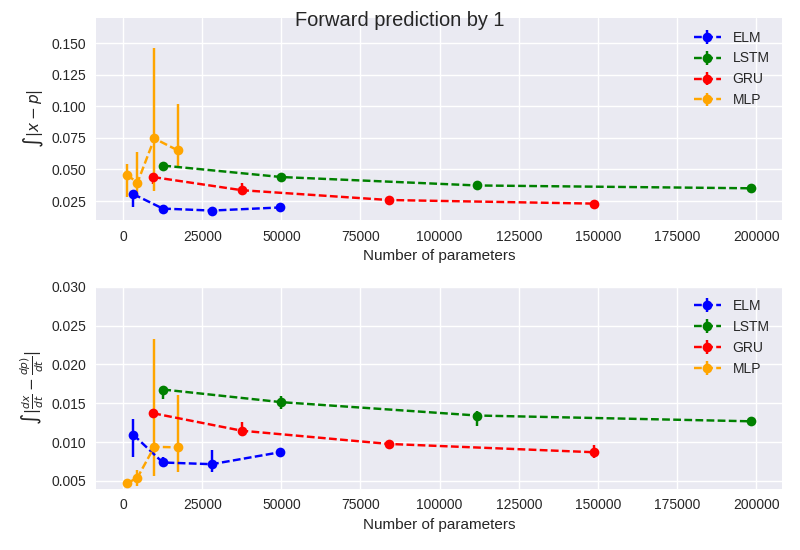
\includegraphics[width=.48\textwidth]{figures/mg1_scatter_1.png}
   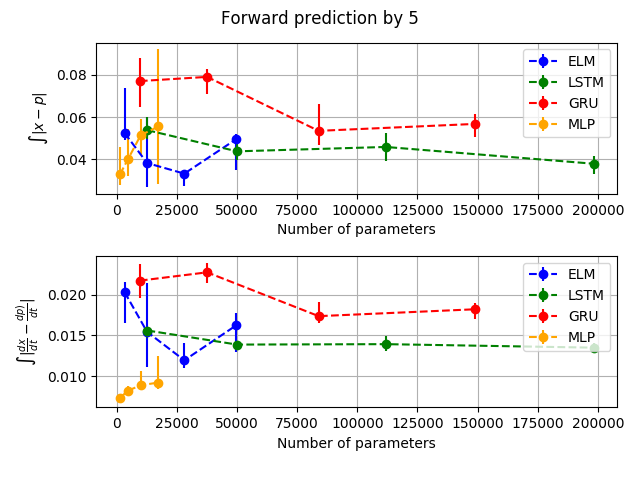
\includegraphics[width=.48\textwidth]{figures/mg1_scatter_5.png}
   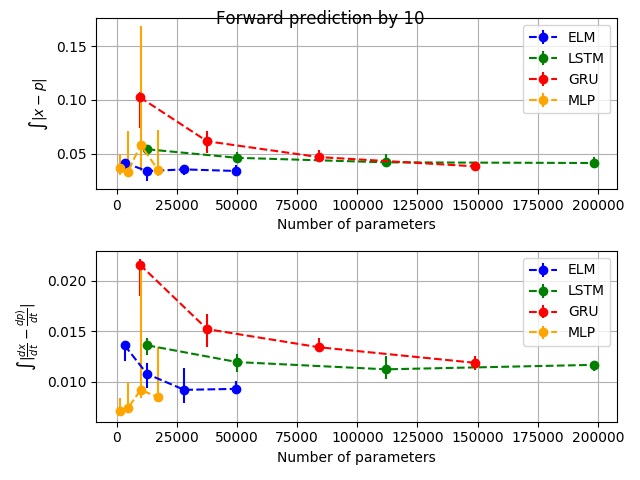
\includegraphics[width=.48\textwidth]{figures/mg1_scatter_10.png}
   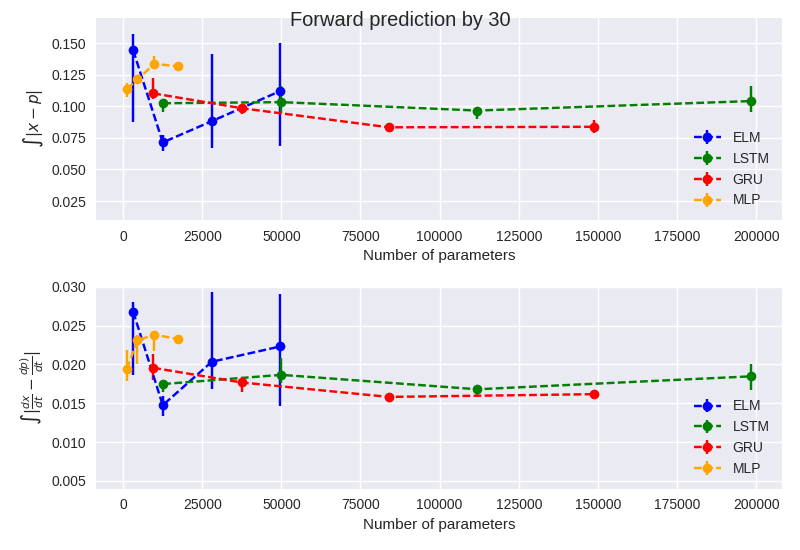
\includegraphics[width=.48\textwidth]{figures/mg1_scatter_30.png}
    
    \caption{Scatter plots showing model performance with respect to
      number of parameters. Using 10 evaluations with different weight
    initializations, points show the median with vertical bars
    extending 1 quartile above and below the median. From left to
    represent the models with hidden nodes of 32, 64, 96, and 128.}
    \label{fig:mg1}
    \end{center}
  \end{figure}


 \subsection {Varying MG Parameters}
 In this experiment, i used the gated models with hidden node sizes
 of 128. Again, i attempted forecasting with $t_0$ = 1, 5, and 10,
 varying randomized 1, 2, or 3 of (params). The parameter degredation
 scatter plot can be found in figure N.

 Sample figures are hidden nodes of 64
 \section{Conclusion}

% \appendices{}
  
 \begin{figure}
   \begin{center}
   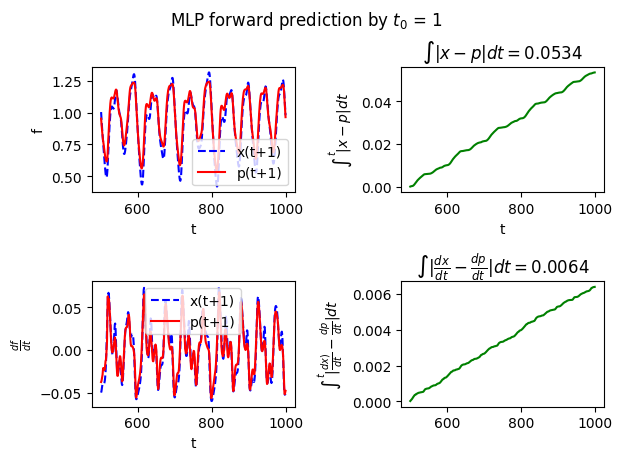
\includegraphics[width=.48\textwidth]{figures/MLP_1.png}
   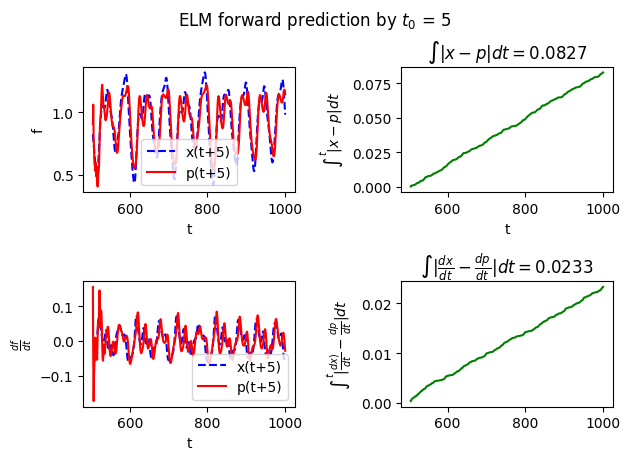
\includegraphics[width=.48\textwidth]{figures/ELM_5.png}
   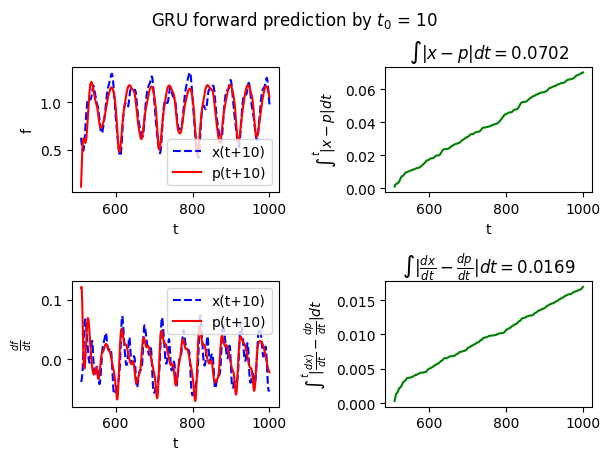
\includegraphics[width=.48\textwidth]{figures/GRU_10.png}
   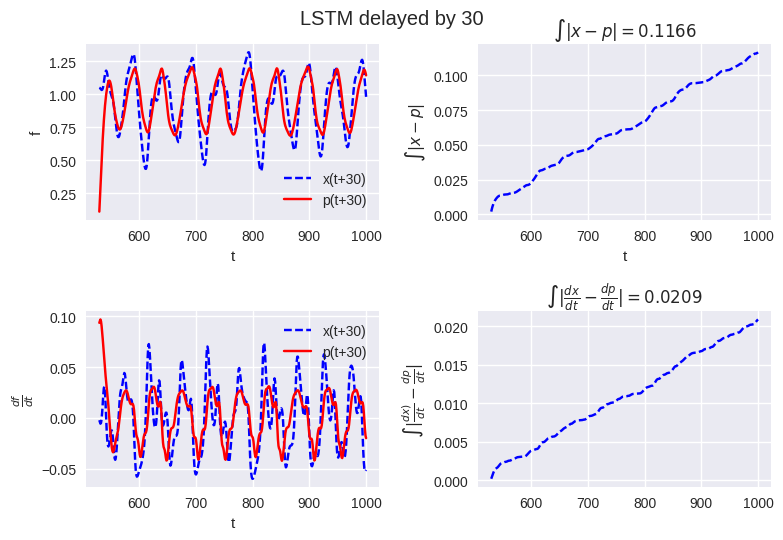
\includegraphics[width=.48\textwidth]{figures/LSTM_30.png}
 \end{center}
 \caption{Sample Curve fittings for MLP, ELM, GRU, and LSTM with
   delays of 1, 5, 10, and 30 respectively. The predicted and true
   values of the functions and slopes are plotted, along with the
   cumulative absolute differences. Note how the cumulative
   differences begin large and increase constantly throughout the evaluation.}
 \label{fig:func_evals}
   \end{figure}

\end{document}
